\documentclass[12pt,a4paper]{article}

\usepackage{fontspec}
\XeTeXlinebreaklocale "th"
\XeTeXlinebreakskip = 0pt plus 1pt
\defaultfontfeatures{Ligatures=TeX}
\setmainfont[
  Path={fonts/TH Sarabun PSK V-1/},
  Extension=.ttf,
  UprightFont={*},
  BoldFont={* Bold},
  ItalicFont={* Italic},
  BoldItalicFont={* BoldItalic}
]{THSarabun}
\setmonofont{Latin Modern Mono}

\usepackage{amsmath,amssymb,mathtools}
\setcounter{MaxMatrixCols}{24}
\usepackage{graphicx,float,caption,subcaption,xcolor,hyperref,fancyhdr}
\usepackage{geometry,booktabs,array,tabularx,longtable,pdflscape}
\usepackage{tikz}
\usetikzlibrary{positioning,arrows.meta,calc,shapes.geometric}
\geometry{margin=0.82in}
\setlength{\headheight}{15pt}
\pagestyle{fancy}\fancyhf{}
\lhead{IEEE 14-bus: SG/GFM/GFL --- PF, SSSA และ TS}
\rhead{\thepage}
\hypersetup{colorlinks=true,linkcolor=blue,urlcolor=blue,citecolor=blue}
\renewcommand{\arraystretch}{1.16}
\captionsetup[table]{skip=6pt}
\emergencystretch=2em
\linespread{1.12}
\renewcommand{\abstractname}{บทคัดย่อ}
\renewcommand{\contentsname}{สารบัญ}
\renewcommand{\figurename}{รูปที่}
\renewcommand{\tablename}{ตารางที่}
\renewcommand{\refname}{เอกสารอ้างอิง}

\newcommand{\code}[1]{\texttt{\detokenize{#1}}}
\newcommand{\src}{\textcolor{blue!65!black}{\textbf{SOURCE\_DEFINED}}}
\newcommand{\caseval}{\textcolor{violet!70!black}{\textbf{CASE\_DEFINED}}}
\newcommand{\derived}{\textcolor{teal!70!black}{\textbf{PROJECT\_DERIVED}}}
\newcommand{\numeric}{\textcolor{orange!80!black}{\textbf{NUMERICAL\_METHOD}}}
\newcommand{\pending}{\textcolor{red!75!black}{\textbf{PENDING IMPLEMENTATION/VERIFICATION}}}
\newcommand{\designonly}{\textcolor{purple!75!black}{\textbf{DESIGN\_ONLY}}}
\newcommand{\notapp}{\textcolor{gray!75!black}{\textbf{NOT APPLICABLE}}}
\newcommand{\clamp}{\operatorname{clamp}}
\newcommand{\hold}{\operatorname{conditional\_hold}}

\title{\textbf{ระบบ IEEE 14-bus แบบผสม SG/GFM/GFL}\\
\large สมการไดนามิก, Power Flow, Full-State SSSA และ Time-Domain Simulation\\[2mm]
\normalsize รายงานฉบับร่างที่ยึด Source และ Index Traceability}
\author{In-house Power-flow Project}
\date{18 กรกฎาคม 2569}

\begin{document}
\maketitle

\begin{center}
\fcolorbox{red!70!black}{red!4}{%
\begin{minipage}{0.91\textwidth}
\centering
\textbf{สถานะเอกสาร: SOURCE-TRACEABLE DESIGN DRAFT}\par
รายงานนี้ใส่เฉพาะสมการและสัญญาที่ตรวจสอบย้อนกลับได้แล้วสำหรับ SG,
GFM REGFM\_B1, GFL WECC, composite DAE, modal analysis และ TS
พร้อมเสนอ nonlinear positive-sequence GFL ที่มี PLL และ current states จริงจาก
Yazdani--Iravani, Teodorescu--Liserre--Rodríguez และ Bacha--Munteanu--Bratcu
ส่วนโมเดล GFL ใหม่นี้ยังเป็น \designonly{} และผลเชิงตัวเลข PF/SSSA/TS
ยังรอ implementation/verification โดยจะไม่ถูกแต่งขึ้นเพื่อให้รายงานดูสมบูรณ์
\end{minipage}}
\end{center}

\begin{abstract}
รายงานนี้วางโครงสร้างการวิเคราะห์ระบบ IEEE 14-bus ที่ประกอบด้วยเครื่องกำเนิดซิงโครนัส
(SG), อินเวอร์เตอร์ grid-forming แบบ virtual synchronous machine (GFM--VSG)
และอินเวอร์เตอร์ grid-following (GFL) โดยใช้สมการ production ชุดเดียวกันสำหรับ
การสร้าง equilibrium, การ linearise แบบ full-KCL small-signal stability analysis
(SSSA) และการ integrate แบบ time-domain simulation (TS) จุดสำคัญของรายงานคือ
ทุกผลลัพธ์ต้องย้อนกลับไปยัง bus, device, local/global state index, สมการ และ source
ได้อย่างชัดเจน โมเดล GFM ปัจจุบันคือ REGFM\_B1 จำนวน 13 states ส่วนโมเดล GFL
production ปัจจุบันคือ WECC REGC\_A/REEC\_A จำนวน 7 states ซึ่งไม่มี explicit PLL
รายงานฉบับนี้จึงแยกอย่างเคร่งครัดระหว่างโมเดล WECC production กับแบบจำลอง
PLL-resolved GFL ที่เสนอจากตำรา แบบจำลองใหม่นี้มี ODE, state order, frame,
current injection และ equilibrium map ครบในระดับออกแบบ แต่จะไม่กล่าวอ้าง
GFL PLL participation หรือผล production จนกว่าจะ implement และผ่าน Phase 4--5
\end{abstract}

\newpage
\tableofcontents
\newpage

\section{ขอบเขต สถานะ และ Source Discipline}

หลักการสำคัญคือ production PF, equilibrium, SSSA และ TS ใช้ project-owned
base-MATLAB code ไม่ใช้ external nonlinear solver และไม่รับค่าจากโปรแกรมอ้างอิง
กลับเข้าสู่ production state สมการหรือพารามิเตอร์ทุกตัวต้องจัดประเภทก่อนดูผล:

\begin{table}[H]\centering
\caption{การจำแนกข้อมูลและการตัดสินใจ}
\begin{tabularx}{\textwidth}{>{\bfseries}p{.24\textwidth}X}
\toprule
ประเภท & ความหมาย \\\midrule
SOURCE\_DEFINED & สมการหรือค่าที่ถอดจาก primary source โดยตรง \\
CASE\_DEFINED & ข้อมูลที่ระบุโดย IEEE14/resource configuration หรือ profile ที่ freeze ก่อนรัน \\
PROJECT\_DERIVED & การแปลง base, initialization หรือ algebraic map ที่พิสูจน์จากสมการต้นทาง \\
NUMERICAL\_METHOD & วิธีแก้สมการ, FD step, tolerance, ordering หรือ display convention \\
ASSUMED\_DIAGNOSTIC & สมมติฐานเพื่อวินิจฉัยเท่านั้น ห้ามใช้รองรับ readiness claim \\
\bottomrule
\end{tabularx}
\end{table}

\begin{table}[H]\centering
\caption{สถานะส่วนประกอบ ณ source tree ปัจจุบัน}
\begin{tabularx}{\textwidth}{p{.25\textwidth}p{.27\textwidth}X}
\toprule
ส่วนประกอบ & สถานะ & ข้อจำกัด \\\midrule
GFM REGFM\_B1 & 13-state production model & มี VSG, PLL, filters และ dynamic angle bounds \\
GFL WECC REGC\_A/REEC\_A & 7-state production model & ไม่มี explicit PLL state \\
Modal analysis & standalone consumer ของ $A$ & ไม่แก้ $A_{\rm red}$ หรือ physical quotient construction \\
PLL-resolved nonlinear GFL & \designonly & source set ปิด core ODE gap; ยังไม่เข้า production routing \\
ผล PF/SSSA/TS ในรายงานนี้ & \pending & ต้องสร้างจาก fingerprint เดียวกันหลัง Phase 4--5 \\
Readiness & NOT\_READY & ห้ามกล่าวอ้าง PRODUCTION\_READY/VALIDATED \\
\bottomrule
\end{tabularx}
\end{table}

\subsection{ชุดเอกสารที่ใช้สร้างสมการ GFM/GFL}

รายงานไม่ได้รวมสมการจากทุกไฟล์ที่ค้นพบโดยไม่มีการคัดเลือก แต่กำหนดหน้าที่ของ
แต่ละ source ก่อนสร้างแบบจำลอง ตาราง~\ref{tab:model-sources} คือ source hierarchy
ที่ใช้จริง ส่วนบทความเปรียบเทียบ transient, predictive control และ LCL digital-delay
ใช้สำหรับอภิปรายผลเท่านั้น ไม่ใช่ผู้กำหนด production ODE

\begin{longtable}{p{.20\textwidth}p{.26\textwidth}p{.37\textwidth}}
\caption{Source hierarchy สำหรับ dynamic equations}\label{tab:model-sources}\\
\toprule
Source & ขอบเขตที่นำมาใช้ & สมการ/บทที่เป็นเจ้าของ \\\midrule
\endfirsthead
\toprule Source & ขอบเขตที่นำมาใช้ & สมการ/บทที่เป็นเจ้าของ \\\midrule
\endhead
Du et al., REGFM\_B1 & GFM--VSG production & 13-state order, VSG swing, voltage loop, PLL, filters, limits และ current interface \\
Yazdani--Iravani (2010) & nonlinear GFL plant และ controller & dq transform Ch.~4; nonlinear PLL (8.18)--(8.25); $P,Q$ และ current reference (8.39)--(8.44); current plant/PI (8.45)--(8.57) \\
Teodorescu et al. (2011) & SRF--PLL และ grid-current control & Park transform (8.20)--(8.21), PI--VCO SRF--PLL Fig.~8.11, L-filter state model (9.1)--(9.6), Chs.~9, 10, 12 \\
Bacha et al. (2014) & averaged/reduced state-space & dq power (9.1), switched model (9.2), averaged state model (9.3), linearisation (9.4), reduced model (9.5), PI/anti-windup requirement \\
Alassaf et al. (2023) & explicit-state cross-check & high-order PLL states (25), feed-forward/current-controller/inductor states (26); ไม่ใช้ numerical claims เป็น acceptance oracle \\
Li et al. (2023) & mixed GFL/GFM SSSA cross-check & modular full-order small-signal blocks VC/CC/LF/PLL; linear domain เท่านั้น \\
Fu et al. (2024) & port-level diagnostic & linear $[P,Q]$--$[\omega,V]$ transfer model; ไม่ใช่ nonlinear TS source \\
Milano (2010), Mondal et al. (2014) & PF--DAE--SSSA--TS และ modal math & initialization chain, DAE linearisation, time integration, left/right eigenvectors และ participation factors \\
\bottomrule
\end{longtable}

การประกอบสมการจากสามตำรา GFL เป็น \derived{} เพราะไม่มีเล่มเดียวกำหนด
positive-sequence RMS interface, system-base conversion และ project failure semantics
ครบพร้อมกัน อย่างไรก็ตาม ODE แกนหลักทุกตัวมีเจ้าของใน source และการแปลงที่เพิ่มขึ้น
จะแสดงทีละสมการ ไม่ซ่อนอยู่ใน $A$ matrix ที่แต่งขึ้นเอง

\section{คำอธิบายระบบและเส้นทางการคำนวณ}

กรณีเป้าหมายคือ MATPOWER IEEE 14-bus บน $S_{base}=100$ MVA และ
$f_{base}=60$ Hz โดย resource configuration อาจประกอบด้วย SG และ IBR ที่เลือก mode
เป็น GFM หรือ GFL การกำหนดจำนวน GFM/GFL เป็น input ของ configuration ไม่ใช่ผลที่
เดาจาก eigenvalue

\begin{figure}[H]\centering
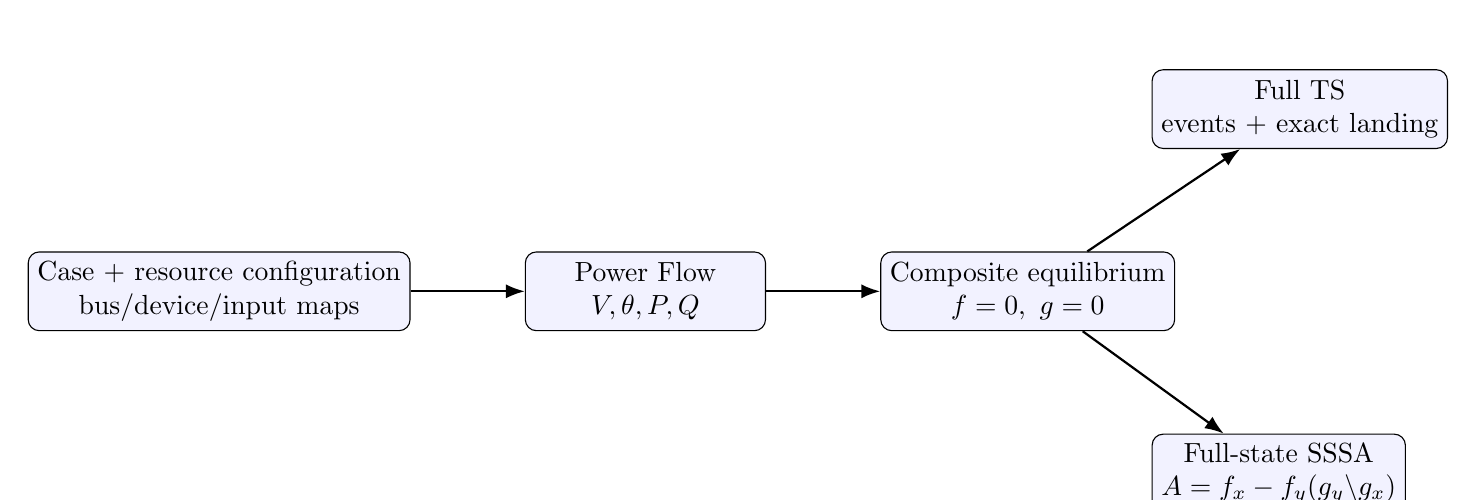
\begin{tikzpicture}[
  box/.style={draw,rounded corners,minimum width=3.05cm,minimum height=1.0cm,align=center,fill=blue!5},
  arr/.style={-{Latex[length=2.4mm]},thick},node distance=1.25cm and 1.45cm]
\node[box] (case) {Case + resource configuration\\bus/device/input maps};
\node[box,right=of case] (pf) {Power Flow\\$V,\theta,P,Q$};
\node[box,right=of pf] (eq) {Composite equilibrium\\$f=0,\ g=0$};
\node[box,below right=1.3cm and -0.3cm of eq] (sssa) {Full-state SSSA\\$A=f_x-f_y(g_y\backslash g_x)$};
\node[box,above right=1.3cm and -0.3cm of eq] (ts) {Full TS\\events + exact landing};
\draw[arr] (case)--(pf); \draw[arr] (pf)--(eq);
\draw[arr] (eq)--(sssa); \draw[arr] (eq)--(ts);
\end{tikzpicture}
\caption{PF, SSSA และ TS ใช้ equilibrium และ state contract ชุดเดียวกัน}
\end{figure}

PF และ SSSA เป็น event-free analysis ส่วน fault, fault clear, SG trip, mode transfer
และ reclose ปรากฏเฉพาะ Full TS หากต้องการ SSSA ของสภาพหลัง trip ต้องสร้าง static
post-trip configuration และหา equilibrium ใหม่ ไม่ใช้ transient sample เป็น equilibrium
โดยไม่มี residual gate

\section{Index และ Traceability Contract}

คำว่า ``index'' ต้องระบุ index space เสมอ เพื่อไม่ให้ Mode No. ถูกตีความเป็น state index
หรือนำ external bus ID ไปใช้เป็นตำแหน่ง array โดยตรง

\subsection{Bus, device และ algebraic indices}

สำหรับ internal bus position $k$,
\begin{equation}
y_{V_R}(k)=2k-1,\qquad y_{V_I}(k)=2k,
\qquad V_k=y_{2k-1}+j y_{2k}.
\end{equation}
คู่ KCL rows ใช้ตำแหน่งเดียวกัน แต่ \code{bus_position} และ \code{bus_id}
ต้องเก็บเป็นคนละ field เพราะ external bus IDs อาจไม่ต่อเนื่อง

\begin{table}[H]\centering\small
\caption{ตัวอย่าง schema ของ resource/device map (ค่าจริงสร้างจาก runtime)}
\begin{tabularx}{\textwidth}{rrrrlrrll}
\toprule
Resource & Device & ID & Bus pos & Bus ID & $x_{start}$ & $x_{end}$ & Type & Mode \\\midrule
-- & -- & -- & -- & -- & -- & -- & -- & -- \\
\bottomrule
\end{tabularx}
\end{table}

\subsection{State, input และ modal indices}

หนึ่ง state ต้องมีอย่างน้อย local state index, global state index,
active-state position และ reduced-state index ใน $A$ หากถูกตัดออกเพราะ inactive,
frozen, fixed active bound หรือ gauge quotient ต้องคงอยู่ใน inventory พร้อมเหตุผล

\begin{table}[H]\centering\scriptsize
\caption{State inventory schema}
\begin{tabularx}{\textwidth}{rrrrllXll}
\toprule
Global $x$ & Active pos & $A$ row & Local $x$ & Device & State & Equation/source & Status & Unit \\\midrule
-- & -- & -- & -- & -- & -- & สร้างจาก metadata registry & -- & -- \\
\bottomrule
\end{tabularx}
\end{table}

สำหรับ SSSA ต้องแยก field ต่อไปนี้ออกจากกัน:
\begin{center}\small
\code{raw_eigen_index}\quad \code{display_mode_number}\\
\code{conjugate_pair_id}\quad \code{eigenvalue_index}
\end{center}
การ sort เพื่อแสดงผลไม่มีสิทธิ์เปลี่ยน association ระหว่าง eigenvector กับ state

\section{Power Flow}

Power flow ใช้ effective bus semantics: REF กำหนด $|V|,\theta$, PV กำหนด $P,|V|$
และ PQ กำหนด $P,Q$ สำหรับ $Y=G+jB$,
\begin{align}
P_i &= |V_i|\sum_{j=1}^{n}|V_j|
\left(G_{ij}\cos\theta_{ij}+B_{ij}\sin\theta_{ij}\right),\\
Q_i &= |V_i|\sum_{j=1}^{n}|V_j|
\left(G_{ij}\sin\theta_{ij}-B_{ij}\cos\theta_{ij}\right),
\end{align}
โดย $\theta_{ij}=\theta_i-\theta_j$ และ Newton step คือ
\begin{equation}
\begin{bmatrix}H&N\\M&L\end{bmatrix}
\begin{bmatrix}\Delta\theta\\\Delta|V|\end{bmatrix}
=\begin{bmatrix}\Delta P\\\Delta Q\end{bmatrix}.
\end{equation}

PF ไม่ได้ integrate dynamic states แต่ให้ operating voltage และ net injection สำหรับ
device equilibrium initializer ตาราง final ต้องแสดงทั้ง specified และ solved quantities,
bus/device indices, mismatch history และ convergence gate

\begin{table}[H]\centering\small
\caption{PF result table --- รอสร้างจาก final operating-point fingerprint}
\begin{tabularx}{\textwidth}{rrlrrrrrrX}
\toprule
Bus pos & Bus ID & Type & $|V|$ & $\theta$ & $P_{spec}$ & $Q_{spec}$ & $P_{sol}$ & $Q_{sol}$ & Status \\\midrule
-- & -- & -- & -- & -- & -- & -- & -- & -- & \pending \\
\bottomrule
\end{tabularx}
\end{table}

\section{Composite DAE และ Equilibrium}

ระบบ production เขียนในรูป input-driven DAE
\begin{equation}
\dot x=f(t,x,y,u,e),\qquad 0=g(t,x,y,u,e;Y),
\label{eq:composite-dae}
\end{equation}
โดย $x$ คือ concatenated device states, $y=[V_R^T,V_I^T]^T$ ตาม interleaved
project ABI, $u$ คือ concatenated named inputs และ $e$ คือ event context
KCL ใช้ generator convention
\begin{equation}
S_i=V_i I_i^*,\qquad P_i=\Re(S_i),\quad Q_i=\Im(S_i),
\end{equation}
โดย $I_i>0$ หมายถึง current injection จาก device เข้าสู่ network

Equilibrium ต้องผ่านทั้ง
\begin{equation}
\|f_{active}(x_0,y_0,u_0,e_0)\|_\infty\le\varepsilon_f,
\qquad
\|g(x_0,y_0,u_0,e_0)\|_\infty\le\varepsilon_g.
\end{equation}
state ที่ frozen ต้องเก็บค่า anchor และไม่ถูกแอบนำเข้า $A_{red}$ ส่วน active bounds
ต้องรายงาน regime เป็น interior/upper/lower ก่อน linearisation

\section{GFM--VSG: REGFM\_B1 จำนวน 13 States}

\subsection{State และ input order}

production state order ที่ freeze แล้วคือ
\begin{equation}
x_{gfm}=\begin{bmatrix}
\omega_m&\delta_{IT}&x_w&x_E&\delta_{PLL}&\xi_{PLL}&
P_f&I_{d,f}&Q_f&V_f&I_{q,f}&\delta_{IT}^{max}&\delta_{IT}^{min}
\end{bmatrix}^{T},
\end{equation}
และ input order คือ $u_{gfm}=[P_{ref},V_{ref}]^T$ บน system base
กำหนด
\begin{equation}
\kappa=\frac{S_{base}}{M_{base}},\qquad
P_{ref,inv}=\kappa P_{ref,sys}.
\end{equation}

\subsection{Reference frame และ current injection}

ใช้ PLL angle แปลง network $xy$ ไป device $dq$:
\begin{align}
I_d&=I_x\cos\delta_{PLL}+I_y\sin\delta_{PLL},&
I_q&=-I_x\sin\delta_{PLL}+I_y\cos\delta_{PLL},\\
V_d&=V_x\cos\delta_{PLL}+V_y\sin\delta_{PLL},&
V_q&=-V_x\sin\delta_{PLL}+V_y\cos\delta_{PLL}.
\end{align}
VSM angle และ voltage-behind-impedance interface คือ
\begin{align}
\delta_{VSM}&=\delta_{PLL}+\clamp(\delta_{IT},\delta_{IT}^{min},\delta_{IT}^{max}),\\
I_{unc}&=\frac{E_{VSM}e^{j\delta_{VSM}}-V}{\kappa(R_e+jX_L)},\\
I&=\begin{cases}
I_{unc},& |I_{unc}|\le I_{maxF}/\kappa,\\
\dfrac{I_{maxF}}{\kappa}\dfrac{I_{unc}}{|I_{unc}|},& |I_{unc}|>I_{maxF}/\kappa.
\end{cases}
\end{align}

\subsection{PLL, VSG, voltage controller และ filters}

เมื่อ $|V|\ge V_{PLLfrz}$,
\begin{align}
\dot\xi_{PLL}&=V_q,\\
\dot\delta_{PLL}&=\omega_0(k_{p,PLL}V_q+k_{i,PLL}\xi_{PLL}),
\end{align}
แต่เมื่อ $|V|<V_{PLLfrz}$ derivatives ทั้งสองถูก freeze เป็นศูนย์
VSG equations ภายใต้ frozen flag profile คือ
\begin{align}
2H\dot\omega_m &= P_{ref,inv}-P_f-\left(\frac{1}{m_p}+D_1\right)\omega_m
-D_2(\omega_m-x_w),\\
\dot x_w&=\omega_D(\omega_m-x_w),\\
\dot\delta_{IT}^{raw}&=\omega_0\omega_m-\dot\delta_{PLL},\\
\dot\delta_{IT}&=\hold(\delta_{IT},\dot\delta_{IT}^{raw},
\delta_{IT}^{min},\delta_{IT}^{max}).
\end{align}
โดย operator ที่ production ใช้จริงเป็น one-sided conditional integration
\begin{equation}
\hold(z,r,\ell,h)=
\begin{cases}
0,&z\ge h\ \text{และ}\ r>0,\\
0,&z\le \ell\ \text{และ}\ r<0,\\
r,&\text{กรณีอื่น},
\end{cases}
\label{eq:gfm-hold}
\end{equation}
ดังนั้น state ที่ชนขอบยังเคลื่อนกลับเข้าด้านในได้ ไม่ใช่การ freeze สองทิศทาง

Voltage controller และ measurement filters คือ
\begin{align}
e_V&=V_{ref}-V_f, &
\dot x_E&=\begin{cases}
0,&E_{raw}\ge E_{max,iq}\ \text{และ}\ e_V>0,\\
0,&E_{raw}\le E_{min,iq}\ \text{และ}\ e_V<0,\\
e_V,&\text{กรณีอื่น},
\end{cases}\\
E_{raw}&=V_{ref}-m_qQ_f+k_{pv}e_V+k_{iv}x_E,
&E_{VSM}&=\clamp(E_{raw},E_{min,iq},E_{max,iq}),\\
T_{pf}\dot P_f&=\kappa P-P_f,&T_{If}\dot I_{d,f}&=\kappa I_d-I_{d,f},\\
T_{Qf}\dot Q_f&=\kappa Q-Q_f,&T_{Vf}\dot V_f&=|V|-V_f,\\
T_{If}\dot I_{q,f}&=\kappa I_q-I_{q,f}.&&
\end{align}
dynamic angle bounds ใช้
\begin{align}
\dot\delta_{IT}^{max}&=\hold(\delta_{IT}^{max},
k_I(I_{d,max}^{SS}-I_{d,f}),0,\delta_{max}),\\
\dot\delta_{IT}^{min}&=\hold(\delta_{IT}^{min},
k_I(-K_eI_{d,max}^{SS}-I_{d,f}),-\delta_{max},0),
\end{align}
เมื่อ $ESFlag=1$ โดย $\delta_{max}=\sin^{-1}(X_LI_{maxSS})$

\subsection{State inventory และ source mapping}

\begin{longtable}{r p{.13\textwidth} p{.25\textwidth} p{.12\textwidth} p{.22\textwidth}}
\caption{REGFM\_B1 13-state order}\label{tab:gfm-states}\\
\toprule
Local & State & Governing relation & Unit & Source/classification \\\midrule
\endfirsthead
\toprule Local & State & Governing relation & Unit & Source/classification \\\midrule
\endhead
1 & $\omega_m$ & VSG swing equation & pu speed deviation & REGFM\_B1 Fig.2; SOURCE\_TRANSFORMED \\
2 & $\delta_{IT}$ & PLL-relative inertial angle with bound hold & rad & Fig.2/Fig.6; PROJECT\_DERIVED hold \\
3 & $x_w$ & damping washout & pu & Fig.2; SOURCE\_TRANSFORMED \\
4 & $x_E$ & voltage PI integral & pu-s & Fig.3; conditional hold PROJECT\_DERIVED \\
5 & $\delta_{PLL}$ & PLL angle & rad & Fig.4; SOURCE\_TRANSFORMED \\
6 & $\xi_{PLL}$ & PLL integrator & pu-s & Fig.4; SOURCE\_TRANSFORMED \\
7 & $P_f$ & active-power filter & pu inverter base & Eq.(1) \\
8 & $I_{d,f}$ & active-current filter & pu inverter base & Eq.(2) \\
9 & $Q_f$ & reactive-power filter & pu inverter base & Eq.(3) \\
10 & $V_f$ & voltage-magnitude filter & pu & Eq.(4) \\
11 & $I_{q,f}$ & reactive-current filter & pu inverter base & Eq.(5) \\
12 & $\delta_{IT}^{max}$ & positive dynamic angle bound & rad & Fig.6; active bound \\
13 & $\delta_{IT}^{min}$ & negative dynamic angle bound & rad & Fig.6; active when $ESFlag=1$ \\
\bottomrule
\end{longtable}

\paragraph{ข้อควรระวังเรื่อง angle identity.}
สมการ $\dot\delta_{VSM}=\omega_0\omega_m$ เป็นจริงเฉพาะ interior unclamped regime
เมื่อ $\delta_{IT}$ ถูก hold ที่ stationary bound จะได้
$\dot\delta_{VSM}=\dot\delta_{PLL}$ และเมื่อ bound เคลื่อนที่ต้องวิเคราะห์ tangent
ของ active regime นั้น ห้ามใช้ smooth identity เดียวครอบทุก regime

\section{GFL ปัจจุบัน: WECC REGC\_A/REEC\_A จำนวน 7 States}

\subsection{State order และ differential equations}

โมเดล canonical GFL ปัจจุบันมี
\begin{equation}
x_{gfl}=\begin{bmatrix}V_{t,f}&P_f&I_{q,cmd,f}&P_{ord}&V_{lvpl,f}&I_{p,reg}&I_{q,reg}\end{bmatrix}^{T},
\quad u_{gfl}=\begin{bmatrix}P_{ref}&Q_{ref}\end{bmatrix}^{T}.
\end{equation}
ODE production คือ
\begin{align}
\dot V_{t,f}&=\frac{|V|-V_{t,f}}{T_{rv}},\\
\dot P_f&=\frac{\kappa P-P_f}{T_p},\\
\dot I_{q,cmd,f}&=\frac{I_{q,cmd}-I_{q,cmd,f}}{T_{iq}},\\
\dot P_{ord}&=\operatorname{rate\_limit}\!\left(
\frac{\clamp(\kappa P_{ref},P_{min},P_{max})-P_{ord}}{T_{pord}},
dP_{min},dP_{max}\right),\\
\dot V_{lvpl,f}&=\frac{|V|-V_{lvpl,f}}{T_{fltr}},\\
\dot I_{p,reg}&=\min\!\left(\frac{I_{p,target}-I_{p,reg}}{T_g},r_{rpwr}\right),\\
\dot I_{q,reg}^{raw}&=\frac{I_{q,cmd,f}-I_{q,reg}}{T_g},\\
\dot I_{q,reg}&=\begin{cases}
\min(\dot I_{q,reg}^{raw},I_{qr,max}),&Q_{ref,inv}>0,\\
\max(\dot I_{q,reg}^{raw},I_{qr,min}),&Q_{ref,inv}<0,\\
\dot I_{q,reg}^{raw},&Q_{ref,inv}=0.
\end{cases}
\end{align}
และ $\operatorname{rate\_limit}(r,r_{min},r_{max})=\clamp(r,r_{min},r_{max})$;
ข้อจำกัดเหล่านี้เป็น derivative limits จึงต้อง linearise ด้วย fixed active regime
เดียวกับที่ equilibrium/TS ใช้
พร้อม directional reactive-current ramp limit ตามเครื่องหมายของ $Q_{ref}$

\subsection{Command, limits และ network current}

กำหนด $V_{div}=\max(V_{t,f},0.01)$ ซึ่งเป็น division guard แบบ
\numeric{} และ
\begin{equation}
I_{p0}=\frac{P_{ord}}{V_{div}},\qquad
I_{q0}=\frac{\kappa Q_{ref}}{V_{div}}+I_{q,inj}.
\end{equation}
เมื่อแรงดันอยู่นอก $[V_{dip},V_{up}]$ จะมี deadband reactive injection
\begin{equation}
I_{q,inj}=\clamp\!\left[K_{qv}\operatorname{deadband}(V_{ref0}-V_{t,f}),
I_{ql1},I_{qh1}\right].
\end{equation}
สำหรับ $PQFlag=1$ ใช้ P-priority circular current limit:
\begin{align}
I_p&=\clamp(I_{p0},0,I_{max}),\\
I_{q,lim}&=\sqrt{\max(I_{max}^2-I_p^2,0)},\\
I_q&=\clamp(I_{q0},-I_{q,lim},I_{q,lim}).
\end{align}
network injection เป็น
\begin{equation}
I=\frac{(I_p-jI_q)e^{j\angle V}}{\kappa}.
\label{eq:wecc-current}
\end{equation}

\begin{longtable}{r p{.16\textwidth} p{.27\textwidth} p{.12\textwidth} p{.2\textwidth}}
\caption{WECC GFL 7-state order}\label{tab:gfl-states}\\
\toprule Local & State & Meaning & Unit & Source/category \\\midrule
\endfirsthead
\toprule Local & State & Meaning & Unit & Source/category \\\midrule
\endhead
1 & $V_{t,f}$ & filtered terminal voltage & pu & REEC\_A measurement filter \\
2 & $P_f$ & filtered electrical active power & pu inverter base & REEC\_A filter \\
3 & $I_{q,cmd,f}$ & reactive-current command lag & pu current & REEC\_A command state \\
4 & $P_{ord}$ & active-power order/rate state & pu inverter base & REEC\_A order state \\
5 & $V_{lvpl,f}$ & LVPL voltage filter & pu & REGC\_A filter \\
6 & $I_{p,reg}$ & active-current regulator state & pu current & REGC\_A regulator \\
7 & $I_{q,reg}$ & reactive-current regulator state & pu current & REGC\_A regulator \\
\bottomrule
\end{longtable}

\paragraph{ข้อจำกัดที่ต้องเขียนตรงไปตรงมา.}
โมเดลนี้ไม่มี $\delta_{PLL}$, PLL integrator, frequency-error integration หรือ
PLL freeze/reset ดังนั้น ``GFL PLL participation'' คือ \notapp{} สำหรับ production
model ปัจจุบัน อย่างไรก็ตาม algebraic orientation $e^{j\angle V}$ ยังทำให้ state
ทั้งเจ็ด couple กับ network angle ได้ จึงห้ามสรุปเชิงโครงสร้างว่า eigenvalues ทุกตัว
ต้องเป็น real poles

\section{PLL-resolved Nonlinear GFL ที่เสนอ}
\label{sec:proposed-gfl}

\begin{center}
\fcolorbox{purple!70!black}{purple!3}{\parbox{.91\textwidth}{
\centering\designonly\par
ส่วนนี้เป็น source-traceable mathematical design ไม่ใช่ production implementation
และไม่เปลี่ยนความหมายของ WECC 7-state model เดิม แบบจำลองใหม่ต้องเป็น opt-in
device คนละชื่อและต้องผ่าน equilibrium, Jacobian, SSSA, TS, limiter และ regression gates
ก่อนนำผลไปอ้างเป็นหลักฐานทางกายภาพ}}
\end{center}

\subsection{ขอบเขตและเหตุผลของ model order}

สำหรับ balanced positive-sequence electromechanical simulation รายงานเลือก
\textbf{GFL--RMS6} เป็นแกนขั้นต่ำที่มี state จริงทุกตัว:
\begin{equation}
x_{gfl6}=\begin{bmatrix}
\delta_{PLL}&\xi_{PLL}&\xi_{id}&\xi_{iq}&i_d&i_q
\end{bmatrix}^{T}.
\label{eq:gfl6-order}
\end{equation}
สอง state แรกเป็น SRF--PLL, สอง state ถัดมาเป็น PI current-controller integrators
และสอง stateสุดท้ายเป็นกระแสจริงของ L-filter ไม่ใช่ measurement states ที่ตั้งชื่อใหม่
DC source ถือว่า stiff และ $P^*,Q^*$ ถูกแปลงเป็น current reference แบบ algebraic
ตาม Teodorescu (8.43)--(8.44) การตัด switching ripple, negative sequence และ LCL resonance
ออกเป็น \derived{} positive-sequence RMS reduction ตามกรอบ averaged model ของ Bacha

หากต้องศึกษาพลังงาน DC และ outer power-control dynamics ให้ใช้
\textbf{GFL--RMS11}:
\begin{equation}
x_{gfl11}=\begin{bmatrix}
\delta_{PLL}&\xi_{PLL}&P_f&Q_f&\xi_P&\xi_Q&
\xi_{id}&\xi_{iq}&i_d&i_q&V_{dc}
\end{bmatrix}^{T}.
\label{eq:gfl11-order}
\end{equation}
RMS11 เป็น extension ที่ต้องมี case data เพิ่ม จึงไม่ใช้แทน RMS6 โดยปริยาย
ส่วน explicit 12-state realization ของ Alassaf et al. ประกอบด้วย PLL realization
หก state, feed-forward สอง state, feedback compensator สอง state และกระแส
$i_d,i_q$ สอง state ใช้เป็น independent structural cross-check แต่ไม่ถูกเลือกเป็น
canonical order เพราะ PLL compensator ลำดับสูงและพารามิเตอร์เป็น study-specific

\subsection{Frame, base, power และ network injection}

ให้ network phasor $V=V_R+jV_I$ อยู่บน system base และให้ PLL angle เป็นมุมสัมพัทธ์
กับ synchronous network frame โดย $\theta_{PLL}=\omega_b t+\delta_{PLL}$
การแปลงไป PLL--dq frameคือ
\begin{align}
v_d&=V_R\cos\delta_{PLL}+V_I\sin\delta_{PLL},\\
v_q&=-V_R\sin\delta_{PLL}+V_I\cos\delta_{PLL},\\
I_{net}&=\frac{(i_d+ji_q)e^{j\delta_{PLL}}}{\kappa},
\qquad \kappa=\frac{S_{base}}{M_{base}}.
\label{eq:gfl-injection}
\end{align}
ด้วย generator convention $S=V\overline I$ จะได้กำลังบน inverter base
\begin{align}
P&=v_di_d+v_qi_q,\\
Q&=v_qi_d-v_di_q.
\label{eq:gfl-pq}
\end{align}
ดังนั้นเมื่อ PLL lock และ $v_q=0$ การฉีด reactive power บวกต้องมี $i_q<0$
เครื่องหมายนี้ต้องถูกทดสอบตรงกับ network KCL ห้ามสลับตามความเคยชินของ load convention

\subsection{Nonlinear SRF--PLL ODE}

Teodorescu Fig.~8.11 และ Yazdani (8.18)--(8.25) ให้ PI phase detector ที่ regulate
$v_q\rightarrow0$ สำหรับ positive-sequence RMS กำหนด
\begin{align}
e_{PLL}&=v_q,\\
\dot\xi_{PLL}&=e_{PLL},\\
\Delta\omega_{PLL}&=k_{p,PLL}e_{PLL}+k_{i,PLL}\xi_{PLL},\\
\dot\delta_{PLL}&=\omega_b\Delta\omega_{PLL},\\
\omega_{PLL}&=\omega_b(1+\Delta\omega_{PLL}).
\label{eq:gfl-pll}
\end{align}
$\delta_{PLL}$ เป็น unwrapped integration state; ค่า wrap mod $2\pi$ ใช้แสดงผลเท่านั้น
และไม่มีสิทธิ์สร้าง discontinuity ใน state หรือ Jacobian ค่า gain ต้องมาจาก case หรือ
ออกแบบจาก bandwidth/damping ก่อนดูผล ไม่ยืมค่าจาก GFM REGFM\_B1 โดยเงียบ ๆ

เมื่อ $|V|<V_{PLL,min}$ ตำราบอกข้อจำกัดของ PLL แต่ไม่กำหนด positive-sequence
LVRT semantics เดียวกัน รายงานจึงกำหนดให้ initialization/transaction \emph{fail closed}
จนกว่า low-voltage freeze/recovery profile จะถูกอนุมัติ การ fail closed นี้เป็น
project safety semantics ไม่ใช่สมการที่อ้างว่า source กำหนด

\subsection{P/Q-to-current reference และ current-priority limit}

Teodorescu (8.43)--(8.44) ให้ $i_d^*=P^*/v_d$ และ $i_q^*=-Q^*/v_d$ เมื่อ
$v_q=0$ รูปทั่วไปที่ได้จากการกลับเมทริกซ์ของสมการ~\eqref{eq:gfl-pq} คือ
\begin{align}
D_V&=v_d^2+v_q^2,\\
i_{d,raw}^*&=\frac{v_dP^*+v_qQ^*}{D_V},\\
i_{q,raw}^*&=\frac{v_qP^*-v_dQ^*}{D_V}.
\label{eq:gfl-iref}
\end{align}
การกลับเมทริกซ์นี้เป็น \derived{} และอนุญาตเมื่อ $D_V\ge V_{div,min}^2$ เท่านั้น
หากต่ำกว่านั้นต้องเข้าสู่ low-voltage failure/approved ride-through route ห้ามใช้
division floor แล้วกล่าวอ้างว่าเป็นพฤติกรรมทางกายภาพ

สำหรับ P-priority circular current limit:
\begin{align}
i_d^*&=\clamp(i_{d,raw}^*,-I_{max},I_{max}),\\
i_{q,max}&=\sqrt{\max(I_{max}^2-(i_d^*)^2,0)},\\
i_q^*&=\clamp(i_{q,raw}^*,-i_{q,max},i_{q,max}).
\label{eq:gfl-current-limit}
\end{align}
Q-priority เป็นคนละ case profile และต้องสลับลำดับอย่างชัดเจน ไม่อนุญาตให้เลือกตามผล

\subsection{Current-controller states, converter voltage และ plant ODE}

กำหนด $R_t=R+R_{on}$ และ current errors
\begin{equation}
e_d=i_d^*-i_d,\qquad e_q=i_q^*-i_q.
\end{equation}
PI states และ raw decoupled commands คือ
\begin{align}
\dot\xi_{id}&=\mathcal A_d(e_d),&u_d&=k_{p,i}e_d+k_{i,i}\xi_{id},\\
\dot\xi_{iq}&=\mathcal A_q(e_q),&u_q&=k_{p,i}e_q+k_{i,i}\xi_{iq},\\
v_{td}^{raw}&=v_d-L\omega_{PLL}i_q+u_d,\\
v_{tq}^{raw}&=v_q+L\omega_{PLL}i_d+u_q.
\label{eq:gfl-controller}
\end{align}
สมการนี้ตรงกับ decoupling ของ Yazdani (8.49)--(8.52) ก่อนใช้กับ converter
ต้องจำกัด modulation vector:
\begin{equation}
\begin{bmatrix}v_{td}\\v_{tq}\end{bmatrix}
=\operatorname{vector\_clamp}
\left(\begin{bmatrix}v_{td}^{raw}\\v_{tq}^{raw}\end{bmatrix},V_{t,max}\right),
\qquad V_{t,max}=m_{max}\frac{V_{dc}}{2}.
\label{eq:gfl-voltage-limit}
\end{equation}
Bacha ระบุว่าต้องมี anti-windup เมื่อ control input ชน limit รายงานใช้
conditional-integration operator
\begin{equation}
\mathcal A(e)=
\begin{cases}
0,&\text{output saturated และ }e\text{ ผลักออกจาก feasible set},\\
e,&\text{interior หรือ }e\text{ ผลักกลับเข้า feasible set}.
\end{cases}
\label{eq:gfl-aw}
\end{equation}
การทดสอบต้องครอบคลุม entry, outward hold, inward release และ opposite-direction recovery

L-filter plant ใช้ nonlinear dq equations ของ Yazdani (8.20)--(8.21):
\begin{align}
L\dot i_d&=L\omega_{PLL}i_q-R_ti_d+v_{td}-v_d,\\
L\dot i_q&=-L\omega_{PLL}i_d-R_ti_q+v_{tq}-v_q.
\label{eq:gfl-current-ode}
\end{align}
เมื่อ voltage command ไม่ saturated การแทน~\eqref{eq:gfl-controller} ลงใน
\eqref{eq:gfl-current-ode} ให้
$L\dot i_d=-R_ti_d+u_d$ และ $L\dot i_q=-R_ti_q+u_q$
แต่ production TS ต้อง integrate สมการเดิมพร้อม actual limited voltage ห้ามใช้รูป decoupled
หลัง saturation เพราะจะซ่อน limiter dynamics

\begin{longtable}{r p{.15\textwidth}p{.30\textwidth}p{.27\textwidth}}
\caption{GFL--RMS6 state order และ equation ownership}\label{tab:gfl6-states}\\
\toprule
Local & State & ODE/meaning & Source/classification \\\midrule
\endfirsthead
\toprule Local & State & ODE/meaning & Source/classification \\\midrule
\endhead
1 & $\delta_{PLL}$ & relative PLL angle, $\dot\delta_{PLL}=\omega_b\Delta\omega_{PLL}$ & Teodorescu Fig.~8.11; Yazdani (8.22)--(8.25); RMS map \derived \\
2 & $\xi_{PLL}$ & PI phase-detector integral & SRF--PLL \src \\
3 & $\xi_{id}$ & d-current PI integral with anti-windup & Yazdani (8.53); Bacha Ch.~9 AW requirement \\
4 & $\xi_{iq}$ & q-current PI integral with anti-windup & same source family \\
5 & $i_d$ & physical L-filter d-current & Yazdani (8.20), Bacha (9.3) \\
6 & $i_q$ & physical L-filter q-current & Yazdani (8.21), Bacha (9.3) \\
\bottomrule
\end{longtable}

\subsection{RMS11 outer loops และ DC-link extension}

สำหรับ state order~\eqref{eq:gfl11-order} เพิ่ม
\begin{align}
T_P\dot P_f&=P-P_f,&T_Q\dot Q_f&=Q-Q_f,\\
e_P&=P^*-P_f,&e_Q&=Q^*-Q_f,\\
\dot\xi_P&=\mathcal A_P(e_P),&
\dot\xi_Q&=\mathcal A_Q(e_Q),\\
i_{d,raw}^*&=i_{d,ff}+k_{pP}e_P+k_{iP}\xi_P,\\
i_{q,raw}^*&=i_{q,ff}-k_{pQ}e_Q-k_{iQ}\xi_Q,
\label{eq:gfl-outer}
\end{align}
โดย $(i_{d,ff},i_{q,ff})$ มาจาก~\eqref{eq:gfl-iref} และเครื่องหมายลบใน q-loop
มาจาก generator reactive-power convention สมการ DC energy balance คือ
\begin{equation}
C_{dc}V_{dc}\dot V_{dc}=P_{dc}-(v_{td}i_d+v_{tq}i_q)-P_{sw,loss}.
\label{eq:gfl-dc}
\end{equation}
ค่า $T_P,T_Q,k_{pP},k_{iP},k_{pQ},k_{iQ},C_{dc}$ และ loss law ต้องเป็น
\caseval{} หรือ source-mapped ก่อนใช้ RMS11 หากไม่มี data ให้ใช้ RMS6 และรายงานว่า
DC/outer-loop dynamics เป็น NOT\_MODELED ห้ามใส่ค่าจำลองเพื่อให้ eigenvalue ดูดี

\subsection{Equilibrium initialization}

จาก PF solution $(V_0,P_0,Q_0)$ ให้
\begin{align}
\delta_{PLL,0}&=\angle V_0,&v_{q0}&=0,&v_{d0}&=|V_0|,\\
i_{d0}&=\frac{P_0}{v_{d0}},&i_{q0}&=-\frac{Q_0}{v_{d0}},\\
\xi_{PLL,0}&=0,&e_{d0}&=0,&e_{q0}&=0,\\
u_{d0}&=R_ti_{d0},&u_{q0}&=R_ti_{q0},\\
\xi_{id,0}&=\frac{u_{d0}}{k_{i,i}},&
\xi_{iq,0}&=\frac{u_{q0}}{k_{i,i}}.
\label{eq:gfl-init}
\end{align}
ก่อนใช้ต้องแปลง $P_0,Q_0$ เป็น inverter base ด้วย $\kappa$ และตรวจย้อนกลับว่า
$I_{net,0}$ จาก~\eqref{eq:gfl-injection} ให้ $V_0\overline I_{net,0}$ ตรง PF injection
หาก voltage command ต้องเกิน $V_{t,max}$, current limit bind หรือ residual ใดไม่ finite
ให้ equilibrium fail closed ไม่ project state เข้า feasible set แบบเงียบ ๆ

สำหรับ RMS11 เพิ่ม $P_{f0}=P_0$, $Q_{f0}=Q_0$, $V_{dc0}=V_{dc}^*$,
$\xi_{P0}=\xi_{Q0}=0$ เมื่อใช้ feed-forward และต้องมี
$P_{dc0}=v_{td0}i_{d0}+v_{tq0}i_{q0}+P_{sw,loss,0}$

\subsection{สมการเดียวกันใน PF, SSSA และ TS}

PF กำหนด $(V_0,P_0,Q_0)$ แต่ไม่ integrate states; equilibrium ใช้
\eqref{eq:gfl-pll}--\eqref{eq:gfl-current-ode} และ~\eqref{eq:gfl-init}
แก้ $f=0,g=0$ พร้อมกัน SSSA differentiate RHS/current injection ชุดเดียวกันใน fixed
active regime ส่วน TS integrate ODE ชุดเดียวกันและใช้ atomic transaction เมื่อ mode,
limit regime หรือ topology เปลี่ยน ไม่มีการสร้าง $A_{GFL}$ แยกขึ้นมาเพื่อรายงาน

ที่ interior unsaturated equilibrium จำนวน GFL--RMS6 eigenvalues ที่เป็นเจ้าของโดย device
เท่ากับหก และ participation ของ $\delta_{PLL},\xi_{PLL},i_d,i_q$ ต้อง trace กลับมายัง
ตาราง~\ref{tab:gfl6-states} ได้ หากใช้ RMS11 จำนวน state เพิ่มเป็นสิบเอ็ดตาม
\eqref{eq:gfl11-order} โดยไม่มีการลบ pole ที่ดูไม่สวย

\section{Fu \texorpdfstring{[P,Q]--[$\omega$,V]}{[P,Q]-[omega,V]} Port Model}

Fu et al. ใช้สำหรับ low/medium-frequency linear diagnostic โดย GFM เขียนเป็น
\begin{equation}
\widetilde v_p=G_b(s)\widetilde v_i^*-Z_b(s)\widetilde S,
\end{equation}
และ GFL เขียนเป็น
\begin{equation}
\widetilde S=G_a(s)\widetilde S^*-Y_a(s)\widetilde v_p.
\end{equation}
PLL closed-loop transfer ใน paper มีรูป
\begin{equation}
G_p(s)=\frac{(k_{p,l}s+k_{i,l})V_{0}}
{s^2+(k_{p,l}s+k_{i,l})V_{0}}.
\end{equation}
realization ของ rational transfer matrix ไม่ unique จึงอาจสร้างได้เฉพาะ
\derived{} + LINEAR\_DIAGNOSTIC\_ONLY และ perturbation states เหล่านั้นห้ามถูก
นำไปเรียกว่า nonlinear production states

นอกจากนี้ Fu ใช้ dynamic RL line/load ใน $Y_{line}(s)$ แต่ production composite DAE
ใช้ algebraic network ดังนั้น whole-system eigenvalues ของ Fu เป็น REFERENCE\_ONLY
การเปรียบเทียบเชิงตัวเลขอนุญาตเฉพาะ converter port ที่ operating point, base, frame
และ network assumption เหมือนกัน

\section{Full-State Small-Signal Stability Analysis}

\subsection{Linearisation และ Schur complement}

ที่ equilibrium $(x_0,y_0,u_0,e_0)$ และ fixed active regime,
\begin{equation}
\begin{bmatrix}\Delta\dot x\\0\end{bmatrix}=
\begin{bmatrix}f_x&f_y\\g_x&g_y\end{bmatrix}
\begin{bmatrix}\Delta x\\\Delta y\end{bmatrix},\qquad \Delta u=0.
\end{equation}
หาก $g_y$ nonsingular,
\begin{equation}
\Delta y=-g_y\backslash(g_x\Delta x),\qquad
A_{full}=f_x-f_y(g_y\backslash g_x).
\end{equation}
จากนั้น project เฉพาะ approved active states:
\begin{equation}
A=A_{full}(\mathcal I_a,\mathcal I_a),\qquad
\#\lambda(A)=|\mathcal I_a|.
\end{equation}
ไม่มีการลบ eigenvalue หลังเรียก \code{eig}

\subsection{Raw domain และ physical decision domain}

\code{sssa.A} คือ full active-state modal domain ส่วน \code{sssa.physical_A}
เป็นอีก domain ที่อาจผ่าน fixed-bound tangent elimination และ common-GFM-PLL gauge
quotient ทั้งสองตารางต้องแสดงพร้อมกันและห้ามเรียก physical-coordinate participation
ว่า original global-state participation จนกว่าจะ lift ผ่าน transformation maps ครบ

\subsection{Eigenvectors และ participation factors}

ให้
\begin{equation}
AV=V\Lambda,\qquad A^HU=U\Lambda^*,
\end{equation}
จับคู่ซ้าย/ขวาแบบ deterministic และ normalize $u_i^Hv_i=1$ จะได้ signed participation
\begin{equation}
p_{ki}=\overline{u_{ki}}v_{ki},\qquad \sum_kp_{ki}\approx1,
\end{equation}
ส่วน nonnegative display ranking คือ
\begin{equation}
\rho_{ki}=\frac{|p_{ki}|}{\sum_j|p_{ji}|}.
\end{equation}
ห้ามเรียก $\rho$ ว่า signed participation หาก repeated/defective cluster ทำให้ individual
participation ไม่ unique ต้องรายงาน UNAVAILABLE\_ILL\_CONDITIONED หรือ subspace-level
result แทนการแต่ง dominant state

\begin{table}[H]\centering\scriptsize
\caption{FULL STATE EIGENVALUES --- schema; ทุก active-state root ต้องปรากฏ}
\begin{tabularx}{\textwidth}{rrr r r r l r r l r r r}
\toprule
No. & Pair & $\Re\lambda$ & $\Im\lambda$ & Hz & $\zeta$ & Device & Global & Local & State & SG\% & GFM\% & GFL\% \\\midrule
-- & -- & \multicolumn{2}{c}{\pending} & -- & -- & -- & -- & -- & -- & -- & -- & -- \\
\bottomrule
\end{tabularx}
\end{table}

display ใช้รูปแบบสองหลักเชิงวิทยาศาสตร์ เช่น
$-7.55\mathrm{e}{-01}+7.32\mathrm{e}{+00}j$ แต่ stored values ต้องคง machine precision
และ Mode No. เป็นเพียง deterministic display number ไม่ใช่ state index

\section{Time-Domain Simulation}

TS integrate สมการเดียวกับ equilibrium และ SSSA ระหว่าง event transactions
สำหรับ implicit trapezoidal,
\begin{equation}
x_{n+1}=x_n+\frac{h}{2}
\left[f(t_n,x_n,y_n,u_n,e_n)+f(t_{n+1},x_{n+1},y_{n+1},u_{n+1},e_{n+1})\right],
\end{equation}
พร้อม endpoint algebraic constraint
\begin{equation}
g(t_{n+1},x_{n+1},y_{n+1},u_{n+1},e_{n+1};Y_{n+1})=0.
\end{equation}

fault on, fault clear, SG trip, GFL/GFM mode transfer และ reclose เป็น atomic
transactions มี left/right samples, transaction ID, pre/right KCL norms และ fail-closed
rollback การลงจอดที่ event time ต้อง exact ไม่ interpolate ข้าม topology discontinuity

\begin{table}[H]\centering\small
\caption{TS event transaction schema}
\begin{tabularx}{\textwidth}{rrlrrrX}
\toprule
Event & Tx & Type & Requested $t$ & Actual $t$ & Bus/device & Status/KCL \\\midrule
-- & -- & -- & -- & -- & -- & \pending \\
\bottomrule
\end{tabularx}
\end{table}

ทุก plot series ต้องมี signal metadata เช่น device ID, bus ID, local/global state index,
symbol, unit, absolute/relative reference และ online/mode interval กราฟที่จะสร้างหลัง
Phase 5 ได้แก่ absolute frequency, fault-bus voltage, device $P/Q$, current magnitude
เทียบ current limit, VSG/PLL angle และ event markers

\section{ผลลัพธ์ที่ต้องสร้างหลัง Phase 4--5}

\begin{table}[H]\centering
\caption{ผลที่ยังไม่ควรถูกเติมด้วยมือ}
\begin{tabularx}{\textwidth}{p{.3\textwidth}Xl}
\toprule
ผลลัพธ์ & หลักฐานที่ต้องมี & สถานะ \\\midrule
PF & case/config fingerprint, iterations, mismatch, bus/branch tables & \pending \\
Equilibrium & active/frozen maps, $\|f\|_\infty$, full KCL, active bounds & \pending \\
Full-state SSSA & $A$ hash/domain, full roots, eigen residuals, participation & \pending \\
Physical spectrum & quotient/tangent maps และ lifted participation & \pending \\
TS & event schedule, accepted steps, residuals, event logs, signal map & \pending \\
Cross-analysis identity & PF/equilibrium fingerprint เดียวกับ SSSA และ TS & \pending \\
\bottomrule
\end{tabularx}
\end{table}

\section{Verification Gates}

\begin{enumerate}
\item ทุก active-state derivative finite และ equilibrium/KCL residual ต่ำกว่า tolerance ที่ freeze ไว้
\item $A_{full}=f_x-f_y(g_y\backslash g_x)$ และ $A$ ตรงกับ approved active projection
\item eigen residual ซ้าย/ขวา, biorthogonality และ participation-sum gates ผ่าน
\item state inventory cardinality ตรงกับ device states และทุก reduced row มี owner เดียว
\item permutation test รักษา eigenvalue multiset และ aggregate device participation
\item PF, SSSA และ TS ใช้ state/input/base/frame/fingerprint เดียวกัน
\item limit tests ครอบคลุม entry, hold, inward release และ opposite-direction recovery
\item ไม่มี \code{inv}, \code{pinv}, external solver หรือ loaded numerical solution ใน production
\item full regression รันหนึ่งครั้งบน final unchanged production tree หลัง Phase 4--5
\end{enumerate}

\section{สถานะหลักฐานปัจจุบัน}

ตาม canonical handoff ณ commit \code{7c72b94}, Phases 0A/1/2/3 และ modal/report
hardening ถูกส่งมอบแล้ว targeted suites รายงาน 77/77 ผ่าน และ full regression ที่
commit \code{80568cf} รายงาน 1024 passed, 0 failed, 4 incomplete โดย incomplete
ทั้งหมดเป็น external PGAz validation assumptions ข้อมูลนี้เป็น provenance จาก handoff
ไม่ใช่การ rerun ใหม่เพื่อสร้างรายงานฉบับนี้ และไม่ใช่หลักฐาน verification ของ
GFL--RMS6/RMS11 ที่เสนอในรายงานฉบับนี้

\section{ข้อจำกัดและงานถัดไป}

\begin{enumerate}
\item GFL WECC ปัจจุบันมี dynamic states จริง แต่ไม่มี explicit PLL state
\item Fu model ใช้อธิบาย linear port behavior ได้ แต่ใช้แทน nonlinear PF/TS model ไม่ได้
\item source set ใหม่ปิด core equation gap สำหรับ GFL--RMS6 ในระดับ \designonly{}
แต่ low-voltage recovery, parameter profile และ positive-sequence limiter semantics
ยังต้อง freeze ก่อน production mutation
\item Phase 4 ต้องสร้าง GFL--RMS6 ใหม่เป็น opt-in model โดยไม่ mutate WECC semantics
\item Phase 5 จึงเชื่อม model เดียวกันเข้าสู่ equilibrium, SSSA และ TS
\item หลัง final gates ผ่าน scripts ต้องสร้าง tables/figures โดยอัตโนมัติและเติมส่วนผลลัพธ์
ของรายงานนี้โดยไม่พิมพ์ตัวเลขด้วยมือ
\end{enumerate}

\section{สรุป}

โครงรายงานและสมการที่ตรวจสอบย้อนกลับได้สำหรับ GFM REGFM\_B1, GFL WECC,
GFL--RMS6/RMS11 ที่เสนอ, PF/equilibrium, full-state SSSA และ TS ถูกจัดวางแล้ว
ในระดับเดียวกับรายงาน Padiyar ชุดตำรา Yazdani, Teodorescu และ Bacha ทำให้สามารถ
ระบุ state order และ nonlinear ODE ของ PLL-resolved GFL ได้โดยไม่แต่ง $A$ matrix
อย่างไรก็ตาม GFL--RMS6/RMS11 ยังเป็น mathematical design ไม่ใช่ production result
จนกว่า implementation และ Phase 4--5 gates จะผ่าน จึงยังไม่มีการกล่าวอ้าง numerical
GFL PLL mode หรือผล PF/SSSA/TS ของโมเดลใหม่

\begin{thebibliography}{9}
\bibitem{regfm}
Du et al., \emph{Grid-Forming Inverter Model Specification: REGFM\_B1},
NREL/TP-5D00-90260, 2024.

\bibitem{wecc2g}
WECC, \emph{Specification of the Second Generation Generic Models for Wind
Turbine Generators}, 2014, REGC\_A and REEC\_A sections.

\bibitem{weccguide}
WECC, \emph{Wind Plant Dynamic Modeling Guidelines}, 2014.

\bibitem{fu2024}
Fu et al., ``A General [P,Q]--[$\omega$,V] Model of Hybrid GFM/GFL Multi-VSC
Systems: Power Oscillation Analysis and Suppression Method,'' IEEE Journal of
Emerging and Selected Topics in Industrial Electronics, 2024.

\bibitem{yazdani2010}
A. Yazdani and R. Iravani, \emph{Voltage-Sourced Converters in Power Systems:
Modeling, Control, and Applications}, Wiley, 2010, Chs.~4 and 8.

\bibitem{teodorescu2011}
R. Teodorescu, M. Liserre, and P. Rodríguez, \emph{Grid Converters for
Photovoltaic and Wind Power Systems}, Wiley, 2011, Chs.~8--12.

\bibitem{bacha2014}
S. Bacha, I. Munteanu, and A. I. Bratcu, \emph{Power Electronic Converters:
Modeling and Control with Case Studies}, Springer, 2014, Chs.~5, 6, and 9.

\bibitem{alassaf2023}
A. Alassaf et al., ``Grid-Following Inverter-Based Resource: Numerical
State--Space Modeling,'' \emph{Sustainability}, vol.~15, 8400, 2023.

\bibitem{li2023}
Y. Li et al., ``Small-signal modelling and stability analysis of grid-following
and grid-forming inverters dominated power system,'' \emph{Global Energy
Interconnection}, vol.~6, no.~3, pp.~363--374, 2023.

\bibitem{milano2010}
F. Milano, \emph{Power System Modelling and Scripting}, Springer, 2010.

\bibitem{mondal2014}
D. Mondal, A. Chakrabarti, and A. Sengupta, \emph{Power System Small Signal
Stability Analysis and Control}, Academic Press, 2014.

\bibitem{contract}
Power-flow Project, \emph{IEEE14 IBR Dynamic Equation Contract},
\path{docs/project/IEEE14_IBR_DYNAMIC_EQUATION_CONTRACT.md}, 2026.
\end{thebibliography}

\end{document}
